\documentclass[aspectratio=169]{beamer}
\usetheme{metropolis}

\usepackage{esdiff}
\usepackage{siunitx}

\usepackage{minted}
\setminted{fontsize=\scriptsize}

\usepackage{circuitikz}
\usetikzlibrary{chains}

\definecolor{blue}{HTML}{005B82}
\definecolor{red}{HTML}{AF5A50}
\definecolor{green}{HTML}{7D966E}
\definecolor{orange}{HTML}{D7AA50}

\title{BrainScaleS Workshop}
\subtitle{4th HBP School}

\date{\today}
\author{Korbinian Schreiber \& Sebastian Billaudelle}
\institute{Kirchhoff-Institute for Physics, Heidelberg University}

\newcommand*\circled[1]{\tikz[baseline=(char.base)]{
	\node[shape=circle,fill=white,draw=mDarkTeal,inner sep=3pt] (char) {\color{white}\textbf{#1}};
	\node[shape=circle,fill=mDarkTeal,inner sep=2pt] (char) {\color{white}\textbf{#1}};
	}}

\begin{document}

\maketitle

\section{Introduction}

{
\usebackgroundtemplate{
\includegraphics[width=\paperwidth]{assets/three_column_background.pdf}}%
\begin{frame}[fragile]
	\frametitle{Analog Neuromorphic Hardware}

	\vspace{-30pt}
	\begin{columns}
		\column{0.33\paperwidth}
		\begin{center}
			\circled{1}
			\vspace{20pt}

			observations
		\end{center}

		\column{0.33\paperwidth}
		\begin{center}
			\circled{2}
			\vspace{20pt}

			mathematical model
		\end{center}

		\column{0.33\paperwidth}
		\begin{center}
			\circled{3}
			\vspace{20pt}

			hardware realization
		\end{center}
	\end{columns}

	\vspace{10pt}

	\begin{columns}
		\column{0.33\paperwidth}
		\begin{center}
			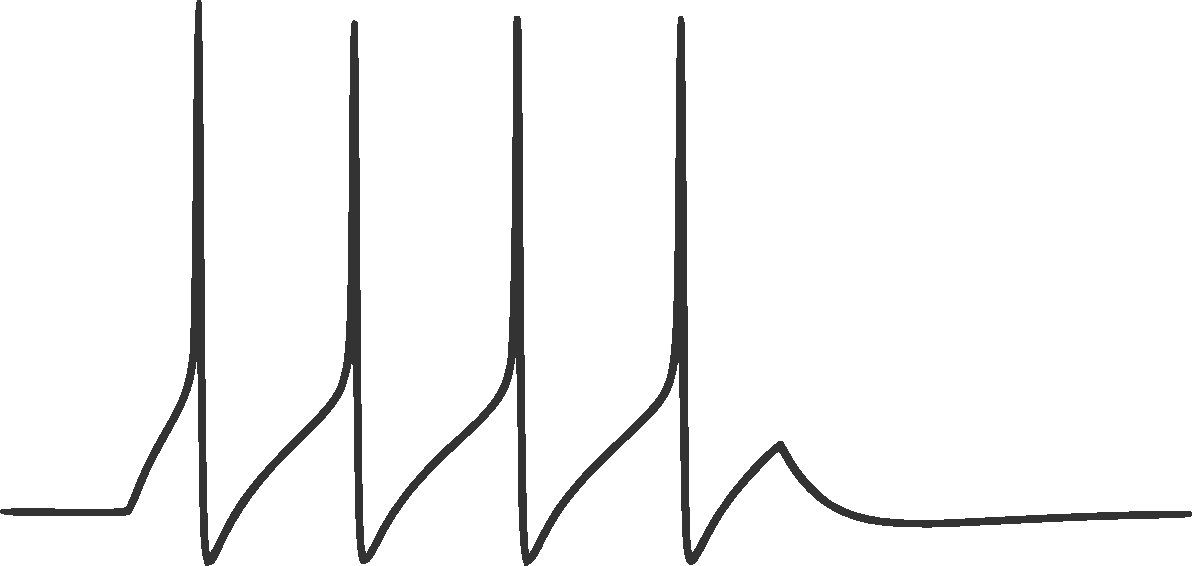
\includegraphics[width=0.8\textwidth]{assets/trace.pdf}
		\end{center}

		\column{0.33\paperwidth}
		\begin{center}
			\vspace{-20pt}
			\begin{gather*}
				\scriptstyle
				C \diff{V}{t} = -g_\text{L} \left( V - E_\text{L} \right) + I_\text{syn}(t) \\
			\end{gather*}
		\end{center}

		\column{0.33\paperwidth}
		\begin{center}
			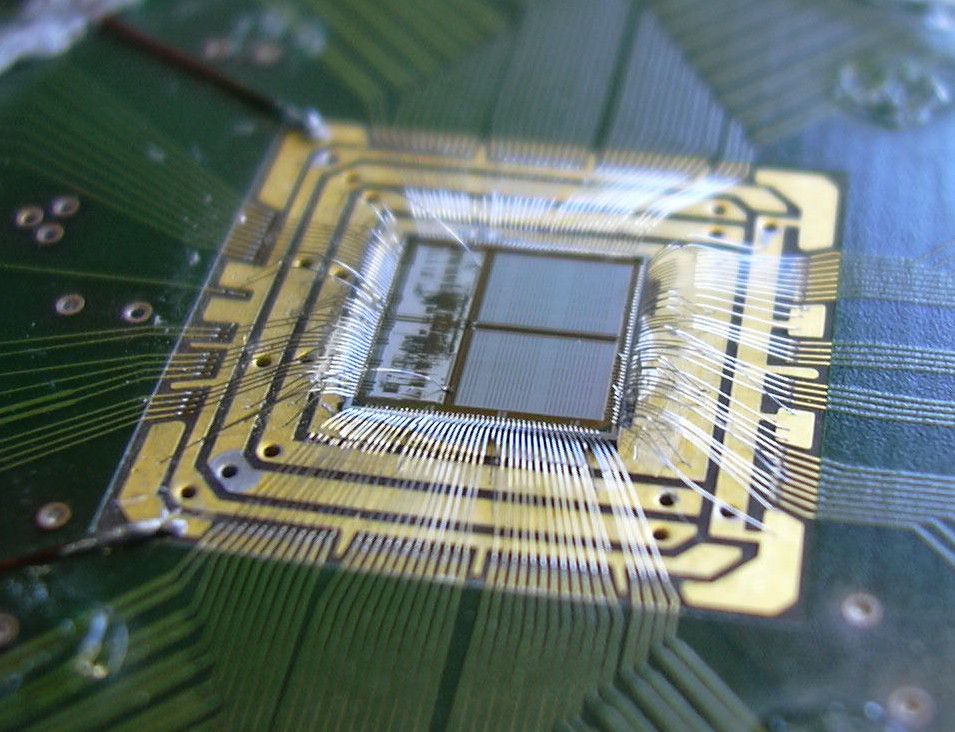
\includegraphics[width=0.8\textwidth]{assets/spikey.jpg}
		\end{center}
	\end{columns}
\end{frame}
}

{
\usebackgroundtemplate{
\includegraphics[width=\paperwidth]{assets/five_column_background.pdf}}%
\begin{frame}[fragile]
	\frametitle{Roadmap}

	\begin{columns}
		\column{0.2\paperwidth}
		\begin{center}
			\circled{2004}
		\end{center}
		\column{0.2\paperwidth}
		\begin{center}
			\circled{2010}
		\end{center}
		\column{0.2\paperwidth}
		\begin{center}
			\circled{2015}
		\end{center}
		\column{0.2\paperwidth}
		\begin{center}
			\circled{2017}
		\end{center}
		\column{0.2\paperwidth}
		\begin{center}
			\circled{2022}
		\end{center}
	\end{columns}

	\vspace{20pt}

	\begin{columns}[T]
		\column{0.2\paperwidth}
		\begin{center}
			\textbf{\color{mDarkTeal}Spikey}
		\end{center}
		\begin{itemize}
				\item single chip system
				\item 384 LIF neurons
		\end{itemize}

		\column{0.2\paperwidth}
		\begin{center}
			\textbf{\color{mDarkTeal}HICANN}
		\end{center}
		\begin{itemize}
				\item \SI{180}{\nano\meter} CMOS
				\item 512 AdEx neurons
		\end{itemize}

		\column{0.2\paperwidth}
		\begin{center}
			\textbf{\color{mDarkTeal}20 Wafer System}
		\end{center}
		\begin{itemize}
			\item 4 million neurons
			\item 0.9 billion synapses
		\end{itemize}

		\column{0.2\paperwidth}
		\begin{center}
			\textbf{\color{mDarkTeal}HICANN DLS}
		\end{center}
		\begin{itemize}
			\item \SI{65}{\nano\meter} CMOS
			\item PPU: integrated processing unit for advanced plasticity
		\end{itemize}

		\column{0.2\paperwidth}
		\begin{center}
			\textbf{\color{mDarkTeal}500 Wafer System}
		\end{center}
		\begin{itemize}
			\item 500 million neurons
			\item 130 billion synapses
		\end{itemize}
	\end{columns}
\end{frame}
}

\begin{frame}{System overview}
	\begin{columns}[onlytextwidth]
		\begin{column}{0.40\textwidth}
			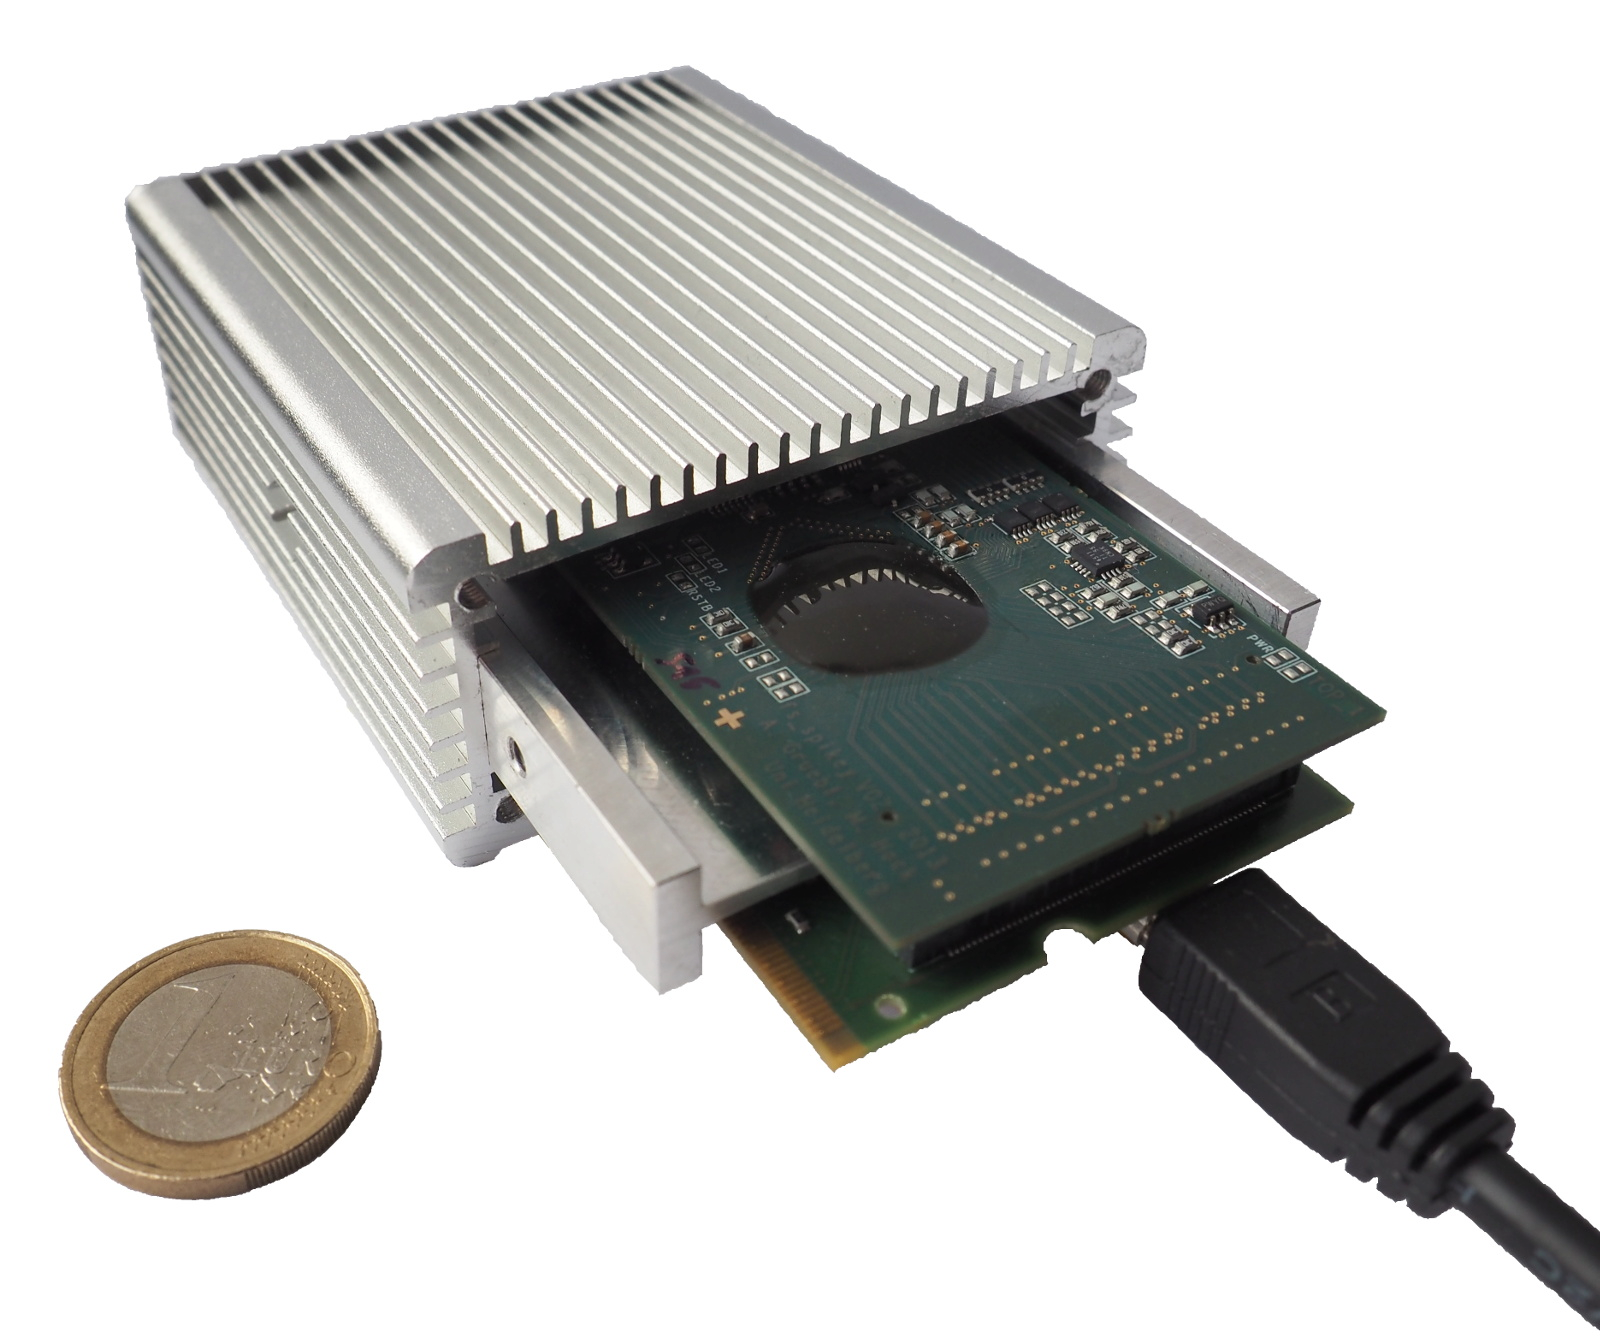
\includegraphics[width=\textwidth]{assets/spikey_system.png}
			\vspace{2ex}
			\begin{center}
				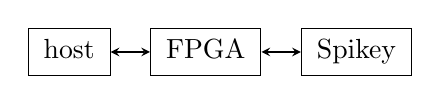
\begin{tikzpicture}[
						start chain,
						node distance=5mm, 
						every node/.style={draw,on chain,join,inner sep=0.6ex,inner xsep=1.3ex}, 
						every join/.style={stealth-stealth}
					]
					\node {\strut host};
					\node {\strut FPGA};
					\node {\strut Spikey};
				\end{tikzpicture}
			\end{center}
		\end{column}
		\hfill
		\begin{column}{0.50\textwidth}
			
			\textbf{Field-programmable gate array:}
			\begin{itemize}
				\item reconfigurable logic gates
				\item experiment control and communication
			\end{itemize}
			
			\vspace{3ex}

			\textbf{Spikey:}
			\begin{itemize}
				\item 384 neurons, 384 $\times$ 256 synapses
				\item speedup of $10^4$
			\end{itemize}
		\end{column}
	\end{columns}
\end{frame}

\begin{frame}{The analog core}
	\begin{columns}[onlytextwidth]
		\begin{column}{0.45\textwidth}
			\begin{tikzpicture}[scale=0.9,transform shape]
				\draw[step=0.5,gray,thin] (0,0) grid ++(5,4);
				\draw[thick] (0,0) rectangle ++(5,4) node[pos=0.5,rectangle,fill=bg] {synapses};
				\foreach \y in {0.25,0.75,...,4.0} {
					\draw (-0.15,\y) -- ++(-0.4,0.23) -- ++(0,-0.46) -- cycle;
					\draw[-stealth] (-1,\y) -- (-0.55,\y);
					\draw[-stealth] (-0.15,\y) -- (0,\y);
				}
				\draw (-1,-1) -- (-1,3.75);

				\draw[step=0.5,gray,thin] (0,-1) grid ++(5,0.5);
				\draw[thick] (0,-1) rectangle ++(5,0.5) node[pos=0.5,rectangle,fill=bg] {neurons};

				\foreach \x in {0.25,0.75,...,5.00}
				\draw[-stealth] (\x,0) -- ++(0,-0.5);
			\end{tikzpicture}
		\end{column}
		\hfill
		\begin{column}{0.50\textwidth}
			\textbf{Synapses:}
			\begin{itemize}
				\item \SI{4}{bit} weights (0…15)
				\item STDP and STP
			\end{itemize}
			
			\vspace{3ex}

			\textbf{Neurons:}
			\begin{itemize}
				\item Leaky-integrate-and-fire model (LIF)
				\item analog parameters can be configured freely
			\end{itemize}
		\end{column}
	\end{columns}
\end{frame}

\begin{frame}{Leaky-integrate-and-fire neurons}
	\begin{columns}[onlytextwidth]
		\begin{column}{0.45\textwidth}
			\begin{align*}
				C_\text{m} \frac{\operatorname{d} V_\text{m}}{\operatorname{d} t} &= - g_\text{l} (V_\text{m} - E_\text{l}) + I_\text{syn} + I_\text{ext}
			\end{align*}

			\vspace{3ex}

			\begin{center}
				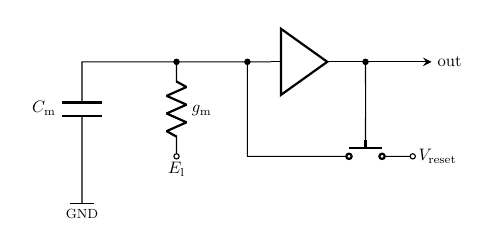
\begin{tikzpicture}[scale=0.6,transform shape]
					\draw (0,0) to[short] ++(0,1)
					to[C,l=$C_\text{m}$] ++(0,2)
					to[short,-*] ++(2,0)
					to[R,l=$g_\text{m}$,-o] ++(0,-2) node[below] {$E_\text{l}$};

					\draw (2,3) to[short] ++(2,0);
					\node[anchor=in,buffer] (comp) at (4,3) {};

					\draw[-stealth] (comp.out) -- ++(2,0) node[right] {out};

					\draw (3.5,3) to[short,*-] (3.5,1)
					to ++(1.5,0)
					to[push button,n=rst,-o] ++(2,0) node[right] {$V_\text{reset}$};

					\draw (comp.out -| rst.north) to[short,*-] (rst.north);

					\draw (0,0) -- ++(-0.25,0) -- node[pos=0.5,below] {\footnotesize GND} ++(0.5,0);
				\end{tikzpicture}
			\end{center}
		\end{column}
	\end{columns}
\end{frame}

\section{Working with Spikey}

\begin{frame}{PyNN API documentation}
	\begin{center}
		\url{https://neuralensemble.org/docs/PyNN/0.7/api/api-0.7.html}
	\end{center}

	\vspace{3ex}

	\textbf{Look out for:}
	\begin{itemize}
		\item \mintinline{Python}{pynn.Population}
		\item \mintinline{Python}{pynn.Projection}
		\item \mintinline{Python}{pynn.*Connector}
	\end{itemize}
\end{frame}

\begin{frame}[fragile]{Creating (groups of) neurons}
	\textbf{Create \emph{populations} of neurons:}
	\begin{minted}{python}
params = {
    "v_thresh": -60.0
    }
neurons = pynn.Population(42, pynn.IF_facets_hardware1, cellparams=params)
	\end{minted}

	\vspace{3ex}

	\textbf{Get a list of default neuron parameters:}
	\begin{minted}{python}
print pynn.IF_facets_hardware1.default_parameters
	\end{minted}
\end{frame}

\begin{frame}[fragile]{Generating stimuli}
	\textbf{Create a stimulus from a spike train:}
	\begin{minted}{python}
spike_train = np.arange(10.0, 101.0, 10.0)
stimulus = pynn.Population(1, pynn.SpikeSourceArray, {"spike_times": spike_train})
	\end{minted}

	\vspace{3ex}

	\textbf{There is also a Poisson spike source:}
	\begin{minted}{python}
poisson_params = {
    "start": 10.0,
    "duration": 100.0,
    "rate": 5.0
    }
stimulus = pynn.Population(1, pynn.SpikeSourcePoisson, poisson_params)
	\end{minted}
\end{frame}

\begin{frame}[fragile]{Synaptic connections}
	\textbf{Connect all pre-synaptic to all post-synaptic neurons:}
	\begin{minted}{python}
weight = 15 * pynn.minExcWeight()
conn = pynn.AllToAllConnector(weights=weight)
proj = pynn.Projection(pre, post, conn)
	\end{minted}

	\vspace{3ex}

	\textbf{Specify connections in a list:}
	\begin{minted}{python}
conn = pynn.FromListConnector([(7, 13, w, d), (42, 0, w, d)])
	\end{minted}

	\vspace{3ex}

	\textbf{Other connectors (look at specification):}
	\begin{columns}[onlytextwidth]
		\column{0.333\textwidth}
		\mintinline{Python}{FixedNumberPreConnector}

		\column{0.333\textwidth}
		\mintinline{Python}{FixedNumberPostConnector}

		\column{0.333\textwidth}
		\mintinline{Python}{FixedProbabilityConnector}
	\end{columns}
\end{frame}

\begin{frame}[fragile]{Recording observables}
	\textbf{Spike times:}
	\begin{minted}{python}
neurons.record()
...
spikes = neurons.getSpikes()
	\end{minted}

	\vspace{3ex}

	\textbf{\emph{Analog} membrane traces:}
	\begin{minted}{python}
pynn.record_v(neurons[0], "")
	\end{minted}
	\begin{itemize}
		\item only \emph{one} analog-to-digital converter (ADC)
		\item[→] one can record a single neuron at a time
	\end{itemize}
\end{frame}

\section{Tasks}

\begin{frame}{Task 1: a single neuron}
	\begin{columns}[onlytextwidth]
		\begin{column}{0.48\textwidth}
			\begin{center}
				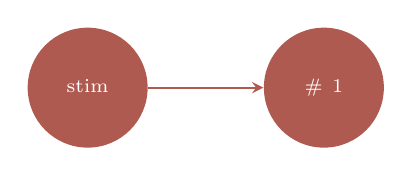
\begin{tikzpicture}
					\node[circle,white,fill=red,text width=1.2cm,align=center] (stm) at (0,0) {\scriptsize\strut stim};
					\node[circle,white,fill=red,text width=1.2cm,align=center] (nrn) at (3,0) {\scriptsize\strut \# 1};

					\draw[-stealth,thick,red] (stm) -- (nrn);
				\end{tikzpicture}
			\end{center}

			\begin{itemize}
				\item create a spike source
				\item create a single LIF neuron
				\item connect these two populations with maximum weight
				\item record spikes and the membrane trace of the stimulated neuron
			\end{itemize}
		\end{column}
		\hfill
		\begin{column}{0.48\textwidth}
			\begin{enumerate}
				\item vary the synaptic weight and observe the membrane trace
				\item play around with the inter-spike interval of the stimulating spike train
				\item observe how the PSPs stack up and eventually cause the neuron to fire
			\end{enumerate}
		\end{column}
	\end{columns}
\end{frame}

\begin{frame}{Task 2: passing spikes}
	\begin{columns}[onlytextwidth]
		\begin{column}{0.48\textwidth}
			\begin{center}
				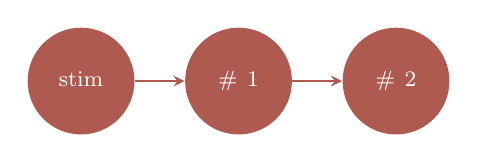
\begin{tikzpicture}
					\node[circle,white,fill=red,text width=1.0cm,align=center] (stm) at (0.0,0) {\footnotesize\strut stim};
					\node[circle,white,fill=red,text width=1.0cm,align=center] (nr1) at (2.0,0) {\footnotesize\strut \# 1};
					\node[circle,white,fill=red,text width=1.0cm,align=center] (nr2) at (4.0,0) {\footnotesize\strut \# 2};

					\draw[-stealth,thick,red] (stm) -- (nr1);
					\draw[-stealth,thick,red] (nr1) -- (nr2);
				\end{tikzpicture}
			\end{center}

			\begin{itemize}
				\item extend the network by adding another neuron
				\item record and plot the spikes of both neurons
			\end{itemize}
		\end{column}
		\hfill
		\begin{column}{0.48\textwidth}
			\begin{enumerate}
				\item think about different possibilities of creating and connecting the neurons
				\item check that the stimulation is passed to the second neuron
			\end{enumerate}
		\end{column}
	\end{columns}
\end{frame}

\begin{frame}{Task 3: a closed synfire chain}
	\begin{center}
		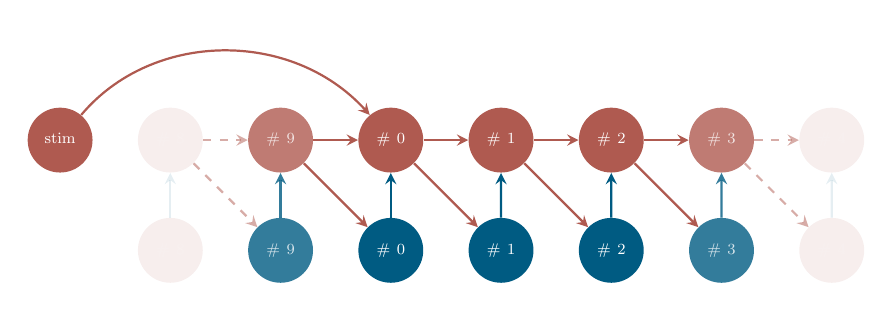
\begin{tikzpicture}[scale=0.7, transform shape]
			\node[circle,white,fill=red,text width=0.8cm,align=center] (stm) at (-4.0,0) {\footnotesize\strut stim};

			\node[circle,white,fill=red,text width=0.8cm,align=center,opacity=0.1] (ex9) at (-2.0,0) {\footnotesize\strut \# 8};
			\node[circle,white,fill=red,text width=0.8cm,align=center,opacity=0.8] (ex10) at (0.0,0) {\footnotesize\strut \# 9};
			\node[circle,white,fill=red,text width=0.8cm,align=center] (ex1) at (2.0,0) {\footnotesize\strut \# 0};
			\node[circle,white,fill=red,text width=0.8cm,align=center] (ex2) at (4.0,0) {\footnotesize\strut \# 1};
			\node[circle,white,fill=red,text width=0.8cm,align=center] (ex3) at (6.0,0) {\footnotesize\strut \# 2};
			\node[circle,white,fill=red,text width=0.8cm,align=center,opacity=0.8] (ex4) at (8.0,0) {\footnotesize\strut \# 3};
			\node[circle,white,fill=red,text width=0.8cm,align=center,opacity=0.1] (ex5) at (10.0,0) {\footnotesize\strut \# 4};

			\node[circle,white,fill=red,text width=0.8cm,align=center,opacity=0.1] (in9) at (-2.0,-2) {\footnotesize\strut \# 8};
			\node[circle,white,fill=blue,text width=0.8cm,align=center,opacity=0.8] (in10) at (0.0,-2) {\footnotesize\strut \# 9};
			\node[circle,white,fill=blue,text width=0.8cm,align=center] (in1) at (2.0,-2) {\footnotesize\strut \# 0};
			\node[circle,white,fill=blue,text width=0.8cm,align=center] (in2) at (4.0,-2) {\footnotesize\strut \# 1};
			\node[circle,white,fill=blue,text width=0.8cm,align=center] (in3) at (6.0,-2) {\footnotesize\strut \# 2};
			\node[circle,white,fill=blue,text width=0.8cm,align=center,opacity=0.8] (in4) at (8.0,-2) {\footnotesize\strut \# 3};
			\node[circle,white,fill=red,text width=0.8cm,align=center,opacity=0.1] (in5) at (10.0,-2) {\footnotesize\strut \# 4};

			% \draw[-stealth,thick,red] (stm) -- (ex1);
			\draw[-stealth,thick,red] (stm) to[out=50,in=130] (ex1);

			\draw[-stealth,dashed,thick,red,opacity=0.5] (ex9) -- (ex10);
			\draw[-stealth,thick,red] (ex10) -- (ex1);
			\draw[-stealth,thick,red] (ex1) -- (ex2);
			\draw[-stealth,thick,red] (ex2) -- (ex3);
			\draw[-stealth,thick,red] (ex3) -- (ex4);
			\draw[-stealth,dashed,thick,red,opacity=0.5] (ex4) -- (ex5);

			\draw[-stealth,dashed,thick,red,opacity=0.5] (ex9) -- (in10);
			\draw[-stealth,thick,red] (ex10) -- (in1);
			\draw[-stealth,thick,red] (ex1) -- (in2);
			\draw[-stealth,thick,red] (ex2) -- (in3);
			\draw[-stealth,thick,red] (ex3) -- (in4);
			\draw[-stealth,dashed,thick,red,opacity=0.5] (ex4) -- (in5);

			\draw[-stealth,thick,blue,opacity=0.1] (in9) -- (ex9);
			\draw[-stealth,thick,blue,opacity=0.8] (in10) -- (ex10);
			\draw[-stealth,thick,blue] (in1) -- (ex1);
			\draw[-stealth,thick,blue] (in2) -- (ex2);
			\draw[-stealth,thick,blue] (in3) -- (ex3);
			\draw[-stealth,thick,blue,opacity=0.8] (in4) -- (ex4);
			\draw[-stealth,thick,blue,opacity=0.1] (in5) -- (ex5);
		\end{tikzpicture}
	\end{center}
		\begin{itemize}
			\item create ten excitatory and ten inhibitory \textbf{populations} of neurons and connect them as depicted
			\item create a transient stimulus to the zeroth excitatory population
			\item record and plot the spikes of the neurons
			\item record the membrane potential of a neuron of your choice
		\end{itemize}
\end{frame}

\begin{frame}{Task 3: a closed synfire chain}
	\begin{enumerate}
		\item evaluate the stability of the chain by tweaking the weight parameters
		\item what happens if you disconnect the inhibitory neurons
		\item modify the chain length
	\end{enumerate}
\end{frame}

\begin{frame}{Task 4: a neural SR latch}
	Think about how to create a simple SR latch (set/reset latch).\\[1em]
	\begin{columns}[onlytextwidth]
		\begin{column}{0.48\textwidth}
			\begin{tabular}{c|c|l}
				S & R & Q \\
				\hline
				0 & 0 & no change \\
				0 & 1 & Q = 0, reset state \\
				1 & 0 & Q = 1, set state \\
				1 & 1 & undefined \\
			\end{tabular}
		\end{column}
		\hfill
		\begin{column}{0.48\textwidth}
			\begin{tikzpicture}[scale=1, transform shape]
				\node[draw,fg,fill=bg,text width=1cm,align=center,minimum height=2.5cm] (latch) at (0,0) {};
				\node[anchor=west] (S) at (-0.7,1) {S};
				\node[anchor=west] (R) at (-0.7,-1) {R};
				\node[anchor=east] (Q) at (0.7,0) {Q};

				\draw[-stealth] (-1.2,1) -- (S);
				\draw[-stealth] (-1.2,-1) -- (R);
				\draw[-stealth] (Q) -- (1.2,0);
			\end{tikzpicture}
		\end{column}
	\end{columns}
\end{frame}

\begin{frame}{Task 4: a neural SR latch}
	\begin{center}
		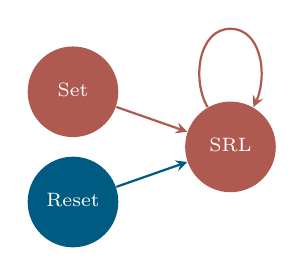
\begin{tikzpicture}[scale=1, transform shape]
			\node[circle,white,fill=red,text width=0.8cm,align=center] (stm_exc) at (0,0.7) {\scriptsize\strut Set};
			\node[circle,white,fill=red,text width=0.8cm,align=center] (srl) at (2,0) {\scriptsize\strut SRL};
			\node[circle,white,fill=blue,text width=0.8cm,align=center] (stm_inh) at (0,-0.7) {\scriptsize\strut Reset};

			\draw[-stealth,thick,red] (stm_exc) -- (srl);
			\draw[-stealth,thick,blue] (stm_inh) -- (srl);
			\draw[-stealth,thick,red] (srl) to[out=120,in=180] (2,1.5) to[out=0,in=60,-stealth] (srl);
		\end{tikzpicture}
	\end{center}
		\begin{itemize}
			\item create a population of latch neurons and project them onto themselfs
			\item create a transient excitatory and a transient inhibitory stimulus to the latch neurons
			\item set the stimuli such that the latch is switched on and off consecutively
			\item record and plot the spikes of the neurons
			\item record the membrane potential of the latch neuron
		\end{itemize}
\end{frame}

\end{document}
